\section{Architetture}

\subsection{Architettura di Von Neumann}
La struttura generale di Von Neumann prevede:

\begin{figure}[H]
    \centering
    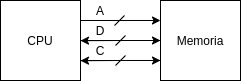
\includegraphics[width=150px]{images/2_Architetture/Von_Neumann.png}
\end{figure}

\begin{itemize}
    \item CPU: central processing unit, si occupa di prendere le istruzioni, decodificarle ed eseguirle
    \item Memoria: contiene i dati e le istruzioni
    \item A: sono i fili di indirizzo, emessi dalla CPU e ricevuti dalla memoria
    \item D: sono i fili di dato, sia la CPU che la memoria possono emettere dati, ovviamente non allo stesso tempo
    \item C: sono i fili di controllo, varia in dimensioni in base alle architetture. Alcuni fili importanti sono il memory\_read, il memory\_write, il segnale di memory\_wait, ecc
\end{itemize}

Alla fine tutto è un numero, anche le istruzioni per la CPU quindi anche le istruzioni possono andare in memoria per Von Neumann.

\subsection{Memoria}
La memoria è genericamente rappresentata come segue:
\begin{figure}[H]
    \centering
    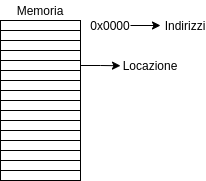
\includegraphics[width=150px]{images/2_Architetture/Memoria.png}
\end{figure}
Si tratta di un insieme di celle dette \emph{locazioni} di memoria, ognuna delle quali ha un \emph{indirizzo}.
Useremo l'esadecimale per indicare gli indirizzi in quanto è semplice convertirli in binario.
Per accedere ad una locazione la CPU emette l'indirizzo sul bus A, se deve scrivere pone anche un dato sul bus D e da il comando di memory\_write, se invece deve leggere pone il comando di memory\_read e campiona il bus D.

Ogni cella è composta da 8 bit per motivi storici: sono abbastanza per memorizzare un singolo carattere secondo la codifica ASCII; ne basterebbero 7 ma è un numero dispari ed anche primo, cosa molto brutta.

Per alcune applicazioni 8 bit possono essere pochi quindi alcuni calcolatori hanno memoria con locazioni di 16 bit, 32 bit, 64 bit.

\subsection{Architettura Harvard}
Per migliorare l'efficienza su alcuni task specifici conviene mettere due memorie separate e di diverso tipo: in questo modo nasce l'architettura Harvard:
\begin{figure}[H]
    \centering
    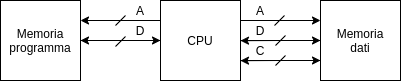
\includegraphics[width=300px]{images/2_Architetture/Harvard.png}
\end{figure}
 L'architttura Harvard è largamente usata per applicazioni DSP - \emph{Digital Signal Processing}, cioè operazioni velocissime e sempre uguali su dati in tempo reale.

\subsection{Comparazione}
\begin{table}[ht]
    \centering
    \begin{tabular}{c|c|c|c|c}
        & Flash & RAM & ALU & Architettura\\
        \hline
        AVR Mega & 128k & 8k & 8bit & Harvard \\
        MSP430 & 65k & 8k & 16bit & Von Neumann \\
        ARM & 1M & 96k & 32 bit & Von Neumann 
    \end{tabular}
\end{table}